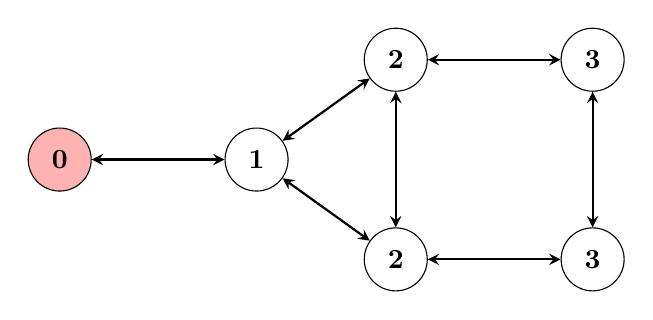
\begin{tikzpicture}[
    >=stealth,
    node distance=2.5cm,
    every node/.style={circle, draw, minimum size=8mm, font=\bfseries},
    edge/.style={draw, thick, <->}
]
    \node[fill=red!30] (S) {0};
    \node (A) [right of=S] {1};
    \node (B) [above right of=A, yshift=-0.5cm] {2};
    \node (C) [below right of=A, yshift=0.5cm] {2};
    \node (D) [right of=B] {3};
    \node (E) [right of=C] {3};

    \path[edge] (S) -- (A);
    \path[edge] (A) -- (B);
    \path[edge] (A) -- (C);
    \path[edge] (B) -- (C);
    \path[edge] (B) -- (D);
    \path[edge] (C) -- (E);
    \path[edge] (D) -- (E);
\end{tikzpicture}
